Die gegebenen Werte der einzelnen Elemente lauten:
\begin{align*}
  L &= (16,8 \pm 0,1) \,\cdot 10^{-3}\Hen \\
  C &= (2,07 \pm 0,01) \,\cdot 10^{-9} \Far \\
  R_1 &= (67,2 \pm 0,2) \Ohm \\
  R_2 &= (682 \pm 1) \Ohm
\end{align*}
Tabelle \ref{tab:amp} zeig die Gemessene Spannungsamplitude in Abhängigkeit der Zeit bei
einer gedämpften Schwingung.
\begin{table}
  \begin{tabular}{c c c c}
    \toprule
    \Delta t/\symup{\si{\micro\second}} & \Delta V/\Volt &
    \Delta t/\symup{\si{\micro\second}} & \Delta V/\Volt \\
    \midrule
     10 & 6,2 & 140 & 2,4  \\
     20 & 5,9 & 150 & 2,0  \\
     30 & 5,4 & 160 & 2,0  \\
     40 & 5,0 & 170 & 1,8  \\
     50 & 4,6 & 180 & 1,7  \\
     60 & 4,3 & 190 & 1,5  \\
     70 & 3,9 & 200 & 1,4  \\
     80 & 3,7 & 210 & 1,3  \\
     90 & 3,3 & 220 & 1,2  \\
    100 & 3,2 & 230 & 1,1  \\
    110 & 2,8 & 240 & 1,0  \\
    120 & 2,8 & 250 & 0,8  \\
    130 & 2,4 & \hrulefill & \hrulefill \\
    \bottomrule
  \end{tabular}
  \caption{Zeitabhäängigkeit der Amplitude}
  \label{tab:amp}
\end{table}

Hieraus ergibt sich dann das Bild, welches in \ref{fig:AMP} zu sehen ist
\begin{figure}[h]
  \centering
  \includegraphics[width=0.8\textwidth]{Bilder/amp.pdf}
  \caption{Einhüllende der gedämpften Schwingung}
  \label{fig:AMP}
\end{figure}
\\
Da $U(t)\propto I(t)$ gilt, ist die Form der Einhüllenden nach Formel
(\ref{eqn:einh}) durch
\begin{equation}
  A = A_0\su{e}^{-2\pi\mu t}
\end{equation}
gegeben.
mit der Ausgleichsrechnung ergeben sich die Werte:
\begin{align*}
  A_0 &= (6,83 \pm 0,05)\Volt\\
  \mu &= (1251,3 \pm 13,6)\,\frac{1}{\sek}.
\end{align*}
Die Werte für $T_\su{ex}$ und $R_\su{eff}$ ergeben sich nach Formel \eqref{eqn:reff}
und \eqref{eqn:tex} und lauten:
\begin{align*}
  R_\su{eff} &= (264 \pm 2)\Ohm \\ % Wert erneut überprüfen
  T_\su{ex}  &= (1,27 \pm 0,01)\,\cdot 10^-4\sek
\end{align*}
Der verbaute Widerstand $R_1$ weicht hier um $195,8\Ohm$ ab.
%Platzhalter für Einhüllende
Ab nun werden andere Elemente mit den Werten
\begin{align*}
  L &= (3,53 \pm 0,03) \,\cdot 10^{-3}\Hen \\
  C &= (5,015 \pm 0,015) \,\cdot 10^{-9} \Far \\
  R_1 &= (30,3 \pm 0,1) \Ohm \\
  R_2 &= (271,6 \pm 0,3) \Ohm
\end{align*}
verwendet.
Der gemessene Wert für den Widerstand $R_\su{ap}$ bei dem der aperiodische Fall
eintritt, beträgt $2,3\cdot 10^3 \Ohm$. Der nach Formel \eqref{eqn:r_ap}
berechnete Wert liegt jedoch bei $(5,700 \pm 0,003)\,\cdot 10^3\Ohm$. Somit ergibt
sich eine Differenzvon $2,4\,\cdot10^3 \Ohm$. Diese Differenz kommt unter anderem durch die Widerstände der
restlichen Bauteile zustande, welche in der Theorie nicht beachtet wurden.
Eine weitere Erklärung für diese Diskrepanz liegt in der Ableseungenauigkeit
des eingestellten Grenzwiderstandes.
Die Daten zur Bestimmung der Resonanzüberhöhung $q$ und die Breite der
Resonanzkurve $\nu_+ - \nu_-$ finden sich in Tabelle \ref{tab:Ucon} wieder.
\begin{table}
  \centering
  \begin{tabular}{c c}
    \toprule
    $\nu/\Hz$ & $U_{ss}$/\Volt \\
    \midrule
     15000 &  8,0  \\
     20000 &  8,1  \\
     25000 & 11,0  \\
     30000 & 14,2  \\
     31000 & 15,0  \\
     32000 & 15,7  \\
     33000 & 16,4  \\
     34000 & 17,0  \\
     35000 & 17,2  \\
     36000 & 17,4  \\
     37000 & 17,1  \\
     38000 & 16,5  \\
     39000 & 15,8  \\
     40000 & 14,9  \\
     45000 & 10,1  \\
     50000 &  7,0  \\
    \bottomrule
  \end{tabular}
  \caption{Kondensatorspannung in Abhängigkeit der Frequenz}
  \label{tab:Ucon}
\end{table}

\\
Die Erregerspannung $U$ beträgt dabei $6,72 \Volt$.
Das Verhältnis $\frac{U_\su{C}}{U}$ wird gegen $\nu$ in einem halblogarithmischen
Diagramm aufgetragen.
\begin{figure}[h]
  \centering
  \includegraphics[width=0.8\textwidth]{Bilder/UcUv.pdf}
  \caption{Normierte Darstellung der normierten Kondensatorspannung}
  \label{fig:UcUv}
\end{figure}
Der Maximalwert $q_\su{exp}$ wird aus dem oberen Graphen als Güte abgelesen. Der
theoretische Wert für die Güte $q_\su{theo}$ wird nach Formel \eqref{eqn:guete} berechnet.
Somit erhält man:
\begin{align*}
  q_\su{exp} &= 2,6 \\
  q_\su{theo} &= 3,09 \pm 0,01
\end{align*}
Daraus ergibt sich eine relative Abweichung von etwa $15\,\si{\percent}$. Um
die Breite der Resonanzfrequenz bestimmen zu können, wird der Frequenzbereich
um das Maximum nun Linear wie in Abbildung \ref{fig:UcUv} im unteren Graphen
zu sehen dargestellt. Die Breite der Resonanzkurve wird abgelesen und mit dem
nach \eqref{eqn:breite} berechnetem Theoriewert verglichen.
\begin{align*}
  (\nu_+ - \nu_-)_\su{exp} &= 10\,\cdot10^3\Hz \\
  (\nu_+ - \nu_-)_\su{theo}&= (12,2 \pm 0,1)\,\cdot 10^3\Hz %Hier nochmal genau nachrechnen
\end{align*}
Daraus ergibt sich eine relative Abweichung von 18\si{\percent}.
Um die Werte der Resonanzfrequenz $\nu_\su{res}$ berechnen zu können, werden
die Daten aus Tabelle \ref{tab:phase} benötigt.
\begin{table}
  \centering
  \begin{tabular}{c c}
    \toprule
    $\nu\,/\kHz$ & $\Delta t\,/\,\su{\si{\micro\second}}$ \\
    \midrule
    15    &    2,4   \\
    20    &    2,4   \\
    25    &    2,4   \\
    30    &    3,2   \\
    31    &    3,8   \\
    32    &    4,2   \\
    33    &    4,8   \\
    34    &    5,0   \\
    35    &    5,6   \\
    36    &    6,2   \\
    37    &    6,6   \\
    38    &    7,2   \\
    39    &    7,8   \\
    40    &    8,0   \\
    45    &    8,8   \\
    50    &    8,4   \\
    55    &    8,0   \\
    \bottomrule
  \end{tabular}
  \caption{Phase in Abhängigkeit der Phase}
  \label{tab:phase}
\end{table}

Diese Daten werden außerdem dazu verwendet um die Frequenzen $\nu_1$ und
$\nu_2$ zu berechnen, an denen die Phase $\frac{\pi}{4}\,\text{beziehungsweise}\,
\frac{3\pi}{4}$ beträgt. Die Phase $\varphi$ wird wie in Abbildung \ref{fig:phse}
zu sehen (halblogarithmisch) gegen die Frequenz $\nu$ aufgetragen.
\begin{figure}[h]
  \centering
  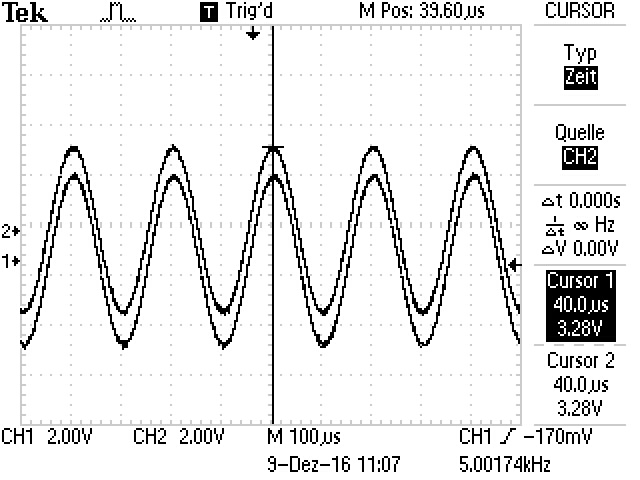
\includegraphics[width=0.8\textwidth]{Bilder/Phase.pdf}
  \caption{Lineare Darstellung der Phasenverschiebung zwischen Erreger- und
  Kondensatorspannung}
  \label{fig:phse}
\end{figure}
Die Frequenz $\nu_\su{res}$ wird nach Formel \eqref{eqn:wres} berechnet
während $\nu_1$ und $\nu_2$ nach Formel \eqref{eqn:w12} berechnet werden.
Die berechneten Werte werden erneut mit den experimentell beobachteten Werten
Verglichen:
\begin{align*}
  \nu_\su{res,exp} &= 36\kHz \\
  \nu_\su{res,theo}&= 36,822 \kHz \\
  \nu_\su{1,exp} &= 29,9\kHz \\
  \nu_\su{1,theo}&=32,19\kHz \\
  \nu_\su{2,exp} &= 42,1 \kHz \\
  \nu_\su{2,theo}&= 69,81\kHz
\end{align*}
Die Werte für $\nu_\su{1,exp}$ und $\nu_\su{2,exp}$ ergeben sich durch
\begin{equation*}
  \nu_\su{res,exp} \pm \frac{1}{2}(\nu_+ - \nu_-)_\su{theo}
\end{equation*}
